\chapter{第1章 绪论}

\section{1.1 研究背景}

小微企业是国民经济的重要组成部分，全国现有约1.2亿户小微市场主体，贡献了50\%以上的税收、60\%以上的GDP和80\%以上的城镇就业\cite{ref1}。然而，小微企业的融资约束问题长期存在，据测算融资缺口约3.8万亿元，融资难、融资贵始终是制约小微主体发展的重要障碍\cite{ref2}。在此背景下，国家将普惠金融上升为核心发展战略，持续推动金融机构加大对小微企业的信贷投放力度。崔惠玉等的研究表明，财政资金的引导作用对地方政府促进小微企业创新具有显著效果\cite{ref4}。王贤彬等的实证研究表明，普惠小微信贷供给对小微企业进入市场具有显著的促进作用，足见金融服务可及性对小微经济活力的基础性影响\cite{ref2}。\par

数字金融的快速发展为缓解小微企业融资约束提供了新的技术路径。Yao和Yang的研究发现，数字金融通过降低信息不对称和交易成本，能够有效缓解中小企业的融资约束\cite{ref6}。祝树金和朱捷尧进一步指出，数字普惠金融不仅扩大了服务覆盖面，还能够推动中小微企业在全球价值链中向上攀升\cite{ref7}。在政策驱动和技术赋能的双重作用下，我国普惠金融领域涌现出一批持牌小微贷款服务机构，行业参与主体涵盖互联网银行、消费金融公司、小额贷款公司和地方性普惠金融平台等多种业态。P公司作为经地方金融监管部门批准的普惠金融公司，并不具备银行牌照，其业务模式专注于为个体工商户和小微企业主提供经营性贷款服务，依托基于大数据的风控模型和半自动化的审批流程，截至研究开展时已积累活跃客户约3,200户，年度业务量约1,860笔，在产品可得性和客群覆盖面上已取得阶段性成果（数据来源：P公司内部业务系统数据）。\par

然而，数字金融在提高覆盖面的同时，也加剧了服务过程中的体验矛盾。行业调研表明，在同类小微贷款服务机构中，产品同质化趋势明显，资金成本与利率水平日趋趋同，客户留存率越来越依赖于服务过程中的体验感知。不同于传统银行依靠物理网点和客户经理长期关系维护的服务模式，普惠金融公司面向的是分散且信息不对称程度高的小微客群，客户在首次接触即面临贷款咨询、材料准备、资质审核、合同签订等多个交互触点，任一个环节的体验断裂都可能导致客户流失。对于小微群体而言，客户对贷款服务的期望已从"能否借到钱"转向"借钱过程是否透明、高效、有温度"。在这一转变中，服务质量成为普惠金融机构差异化竞争的关键维度\cite{ref9}。P公司在快速扩张阶段，服务流程的短板逐步暴露：客户满意度初步测评仅为3.12/5.0（满分为5.0），投诉量年累计约1,024件，投诉有效解决率约为62\%，平均办理时长约为12个工作日，材料一次通过率约为62\%（即首轮提交的贷款申请材料无需补正的客户占比），反映出服务质量与客户期望之间的明显落差。这些现象表明，小微贷款服务质量的改进已不再是锦上添花的辅助动作，而是直接影响客户留存、品牌声誉和风险控制能力的核心管理议题。换言之，服务质量改进是P公司小微贷款业务增长和风险控制的共同抓手。\par

\section{1.2 研究问题提出}

P公司自成立以来，其小微贷款业务流程经历了从线下人工审批向线上化半自动审批的转型。然而，调研数据显示，当前服务流程仍存在若干突出问题。首先，从受理客户的贷款申请到最终放款，办理时长在5至25个工作日之间波动，不同客户经理处理同一类业务的时效差异显著，远超行业标杆机构3至5个工作日的水准。其次，客户提交的贷款申请材料补正率高达28\%，约三成客户在首轮提交后被告知材料不全或信息有误，需要反复往返沟通，不仅延长了办理周期，还加剧了客户的焦虑和不满情绪。第三，客服系统月均接收投诉约85件，涉及客户经理响应延迟、审批进度不透明、还款提醒方式不当等高频问题，其中关于审批进度不透明的投诉占比最大，反映出信息不对称在服务交互中的突出影响。综合来看，客户满意度初测仅为3.12/5.0，处于"基本满意"的下沿，远未达到服务质量管理的行业目标水平。\par

上述痛点反映了小微贷款服务质量管理的三个深层矛盾。其一，服务环节众多、参与角色复杂，贷前咨询、资料审核、风险审批、合同签署、贷后管理等环节之间缺乏统一的服务质量标准，难以系统性地测量和准确定位真实短板。其二，已识别的质量问题往往停留于经验判断层面，管理者依赖直觉分配改进资源，缺少系统性的根因分析工具和方法论支撑，导致改进方向模糊、资源投入分散。其三，已有的改进方案多为一次性的专项行动，缺乏闭环控制和持续监测机制，改进效果难以长期固化和持续优化。汪勇等的研究指出，数字金融场景中的信息不对称依然是制约服务质量的深层根本因素\cite{ref10}。张小敏关于线上贷款流程优化的研究则表明，服务流程碎片化和管理标准缺失是导致客户体验断裂的关键原因\cite{ref11}。上述学术论断与P公司的实践痛点在本质上高度吻合。\par

从工程管理的视角审视，小微贷款服务质量问题本质上是一个可定义、可测量、可分析、可改进和可控制的管理过程变量，而非单纯依靠增加客服投入即可解决的服务态度问题。P公司的服务质量困境呼唤一套兼具系统性和工程化特征的方法论框架，以实现从经验式管理向数据驱动式管理的范式转换。基于上述对P公司服务痛点的诊断和文献参照，本文提出以下四个研究问题：\par

研究问题1：如何构建适用于小微贷款业务场景的服务质量评价模型，系统测量P公司服务质量的表现水平与结构特征？\par

研究问题2：在量化评价的基础上，P公司小微贷款服务质量的核心短板是什么？其深层根因是什么？\par

研究问题3：针对识别的核心短板及其根因，如何设计一套工程化、可落地的服务质量改进方案？\par

研究问题4：如何建立持续监测与控制机制，确保服务质量改进效果能够长期巩固，形成"评价—改进—控制"的管理闭环？\par

上述四个问题构成了一条从问题定位到效果固化的完整问题链：测量服务质量水平（问题1）带动短板与根因的识别（问题2），进而驱动工程化改进方案的设计（问题3），最终建立持续控制的闭环机制（问题4）。这条问题链的逻辑落点始终指向同一个核心命题：服务质量改进是P公司业务增长与风险控制的交汇枢纽。\par

\section{1.3 研究意义}

本研究的理论意义体现在以下两个方面。第一，将服务质量评价理论引入小微贷款这一细分金融服务场景，对SERVQUAL经典模型进行针对性的维度改良，在保留可靠性、响应性、保证性、移情性和有形性五个经典维度的基础上，新增便利性、透明性和产品适配三个维度，构建了包含八个维度的服务质量评价框架，丰富了服务质量理论在普惠金融领域的应用证据。第二，将IPA重要性—绩效分析矩阵与AHP层次分析法进行组合赋权，嵌入DMAIC改进方法的测量与分析阶段，形成了"评价测量—优先级排序—根因追溯"的工程化分析路径，在一定程度上弥补了现有研究中服务质量评价与改进策略之间衔接不足的缺口\cite{ref12}。韩莉等的助贷研究综述指出，当前学术界对金融科技服务质量的系统性优化缺乏方法论探索\cite{ref9}，本研究的理论努力正是对这一研究空白的回应。\par

在实践层面，本研究以P公司为具体案例，产出可直接操作的服务质量诊断方案、改进方案和持续控制机制。对于P公司而言，这意味着能够将客户满意度从3.12分提升至可量化的目标水平，将投诉量从年均1,024件控制在可接受的区间内，将材料补正率从28\%降低至行业合理水平，同时将投诉有效解决率从62\%提升至行业优秀水准，在材料一次通过率维持稳定的前提下实现服务质量的全面升级。对于同类普惠金融服务机构，本研究所构建的DMAIC服务质量改进模式提供了"诊断—测量—改进—控制"的全链路方法论参照，具有较强的可迁移性和实践推广价值。Lu等的研究表明，数字普惠金融对中小企业融资约束的缓解效果在很大程度上取决于服务交付过程中的客户体验质量\cite{ref13}。因此，提升服务质量本身就是深化普惠金融效用的实践逻辑。服务质量改进作为P公司小微贷款业务增长与风险控制的核心交汇点，贯穿本文始终。\par

\section{1.4 研究内容、方法与技术路线}

本文的研究内容围绕前述四个研究问题展开，形成七项递进式任务。（1）P公司服务质量现状诊断：基于业务系统数据提取、客户投诉记录文本分析和内部半结构化访谈，全面扫描服务流程中的质量薄弱环节。（2）SERVQUAL改良服务质量评价模型的构建：在经典五维模型基础上扩展至八个维度，以适应小微贷款服务的信息不对称特征和多角色协同特征\cite{ref14}。（3）基于改良模型的P公司服务质量测量与数据分析：通过面向活跃客户的问卷调研获取各维度的期望值与感知值数据，计算服务质量差距分数。（4）IPA四象限矩阵与AHP组合赋权分析：以IPA识别各服务维度的改进紧迫性，以AHP确定各维度的相对重要权重，定量锁定服务质量的核心短板\cite{ref15}。（5）DMAIC方法框架下的根因分析与改进方案设计：运用鱼骨图、因果矩阵和帕累托分析等质量管理工具，定位短板的深层原因并产出工程化改进方案和试点验证计划\cite{ref12}。（6）改进方案的实施保障体系设计：包括组织架构调整、考核制度配套和信息系统支撑三个层面。（7）持续控制机制的设计与服务质量的闭环管理方案：建立关键质量指标的监测面板和定期评审机制。上述研究任务以DMAIC方法论为逻辑主轴，严格按照"定义—测量—分析—改进—控制"五阶段依次推进，确保从问题界定到效果固化的全流程闭环。\par

在研究方法层面，本文采用以案例研究为核心、问卷调研与统计分析为辅助的混合研究方法，遵循Yin（2018）提出的案例研究设计方法论\cite{ref16}。具体而言：（1）以P公司为单一案例研究对象，通过业务系统数据提取、半结构化访谈、客户投诉文本分析三种途径获取覆盖服务全流程的一手资料。（2）以SERVQUAL改良八维模型为理论原型，设计面向P公司小微贷款客户的服务质量调查问卷，每个维度下设3至5个测量题项，采用李克特五级量表分别采集客户对各项服务属性的期望值与实际感知值。（3）使用SPSS 26.0软件对问卷数据进行信效度分析，以Cronbach's $\alpha$系数检验内部一致性信度，以探索性因子分析验证问卷的结构效度，确保测量工具的科学性和数据采集质量。（4）以IPA四象限分析法为框架，以各维度重要性均值和绩效均值为坐标原点，将八个服务维度映射到四个象限中，同时利用AHP方法邀请P公司管理层和行业专家进行维度两两比较判断和权重计算，形成组合赋权的短板识别图谱。（5）以DMAIC为核心方法论框架，在"定义"阶段明确改进范围与目标指标，在"测量"阶段完成数据采集和当前绩效基线建立，在"分析"阶段使用鱼骨图和因果矩阵进行根因追溯，在"改进"阶段针对根因产出具体的可执行方案及验证计划，在"控制"阶段设计SPC控制图和定期审计机制以确保改进效果的长期维持\cite{ref12}。技术路线如图1-4所示。\par

\begin{figure}[htbp]
  \centering
  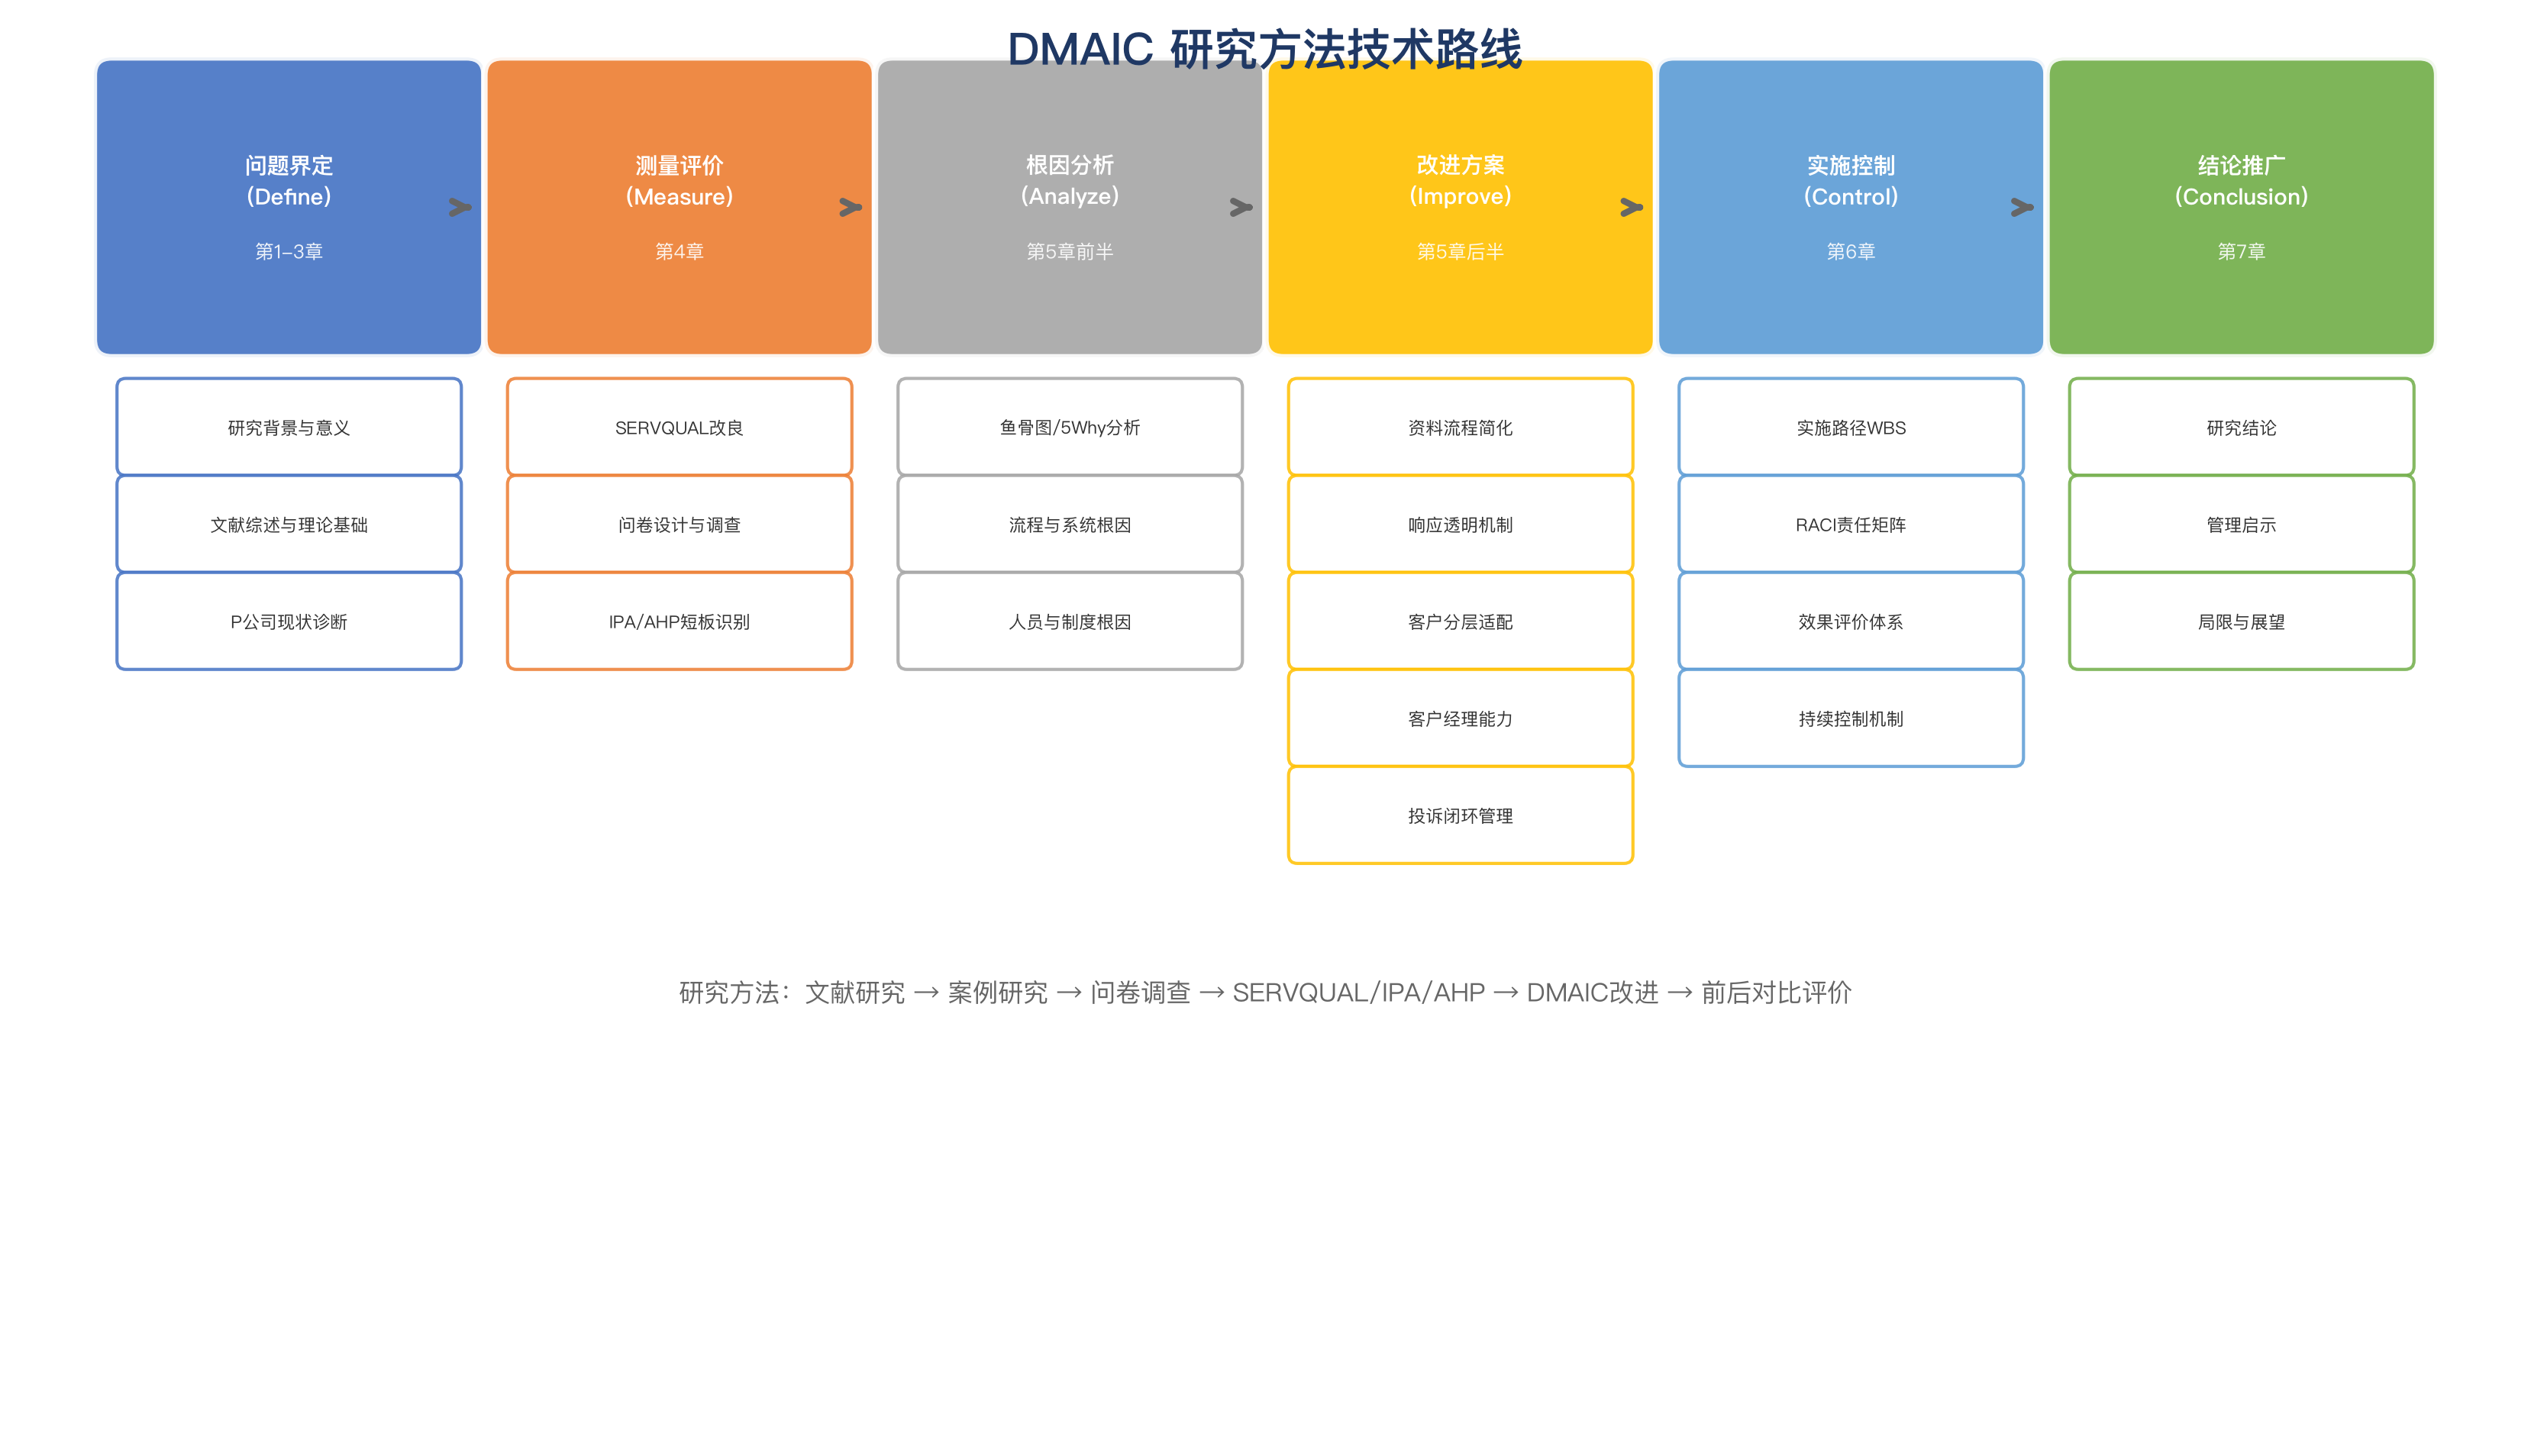
\includegraphics[width=0.85\textwidth]{figures/图1-4_技术路线图.png}
  \caption{本文技术路线图}
  \label{fig:1-4}
\end{figure}

\section{1.5 研究贡献与论文结构}

本研究的主要贡献可归纳为以下四个方面。第一，将服务质量评价研究引入小微贷款这一细分金融服务场景，在经典SERVQUAL五维模型的基础上进行场景化改良，增加了便利性、透明性和产品适配三个维度，形成适用于小微贷款服务特征的八维评价框架，回应了该场景中信息不对称程度高、多角色协同复杂的独特特征，在现有文献中较少被系统探讨。第二，构建了IPA四象限与AHP层次分析的组合赋权方法，以重要性—绩效交叉定位初步识别关键短板维度，以AHP定量权重修正经验判断可能带来的偏差，为小微贷款服务质量的短板识别提供了兼具可视化优势和定量化精度的方法工具。第三，将DMAIC闭环方法论应用于普惠金融服务质量改进领域，使质量评价与改进方案形成有机衔接，避免了传统研究中评价活动与改进活动互相割裂的局限\cite{ref12}。第四，设计了包含组织保障、制度保障和系统保障的三层实施保障体系，以及基于SPC统计过程控制思想的持续监测机制，使服务质量的改进效果具备可长期维持的工程化基础，超越了单一项目式改进的短期局限。\par

本文共分为七章，结构安排如下。第1章（绪论）阐述研究背景、研究问题、研究意义、研究内容与方法、研究贡献、论文结构以及研究局限。第2章（文献综述与理论基础）系统梳理普惠金融与小微贷款、金融科技服务模式、服务质量与客户满意度、SERVQUAL/IPA/AHP方法论以及DMAIC方法的研究现状。第3章（P公司小微贷款服务质量现状诊断）基于业务数据和客户调研，全面扫描并描述P公司服务流程中的质量痛点。第4章（服务质量评价模型的构建与测量）阐述SERVQUAL改良八维模型的设计逻辑与问卷测量结果。第5章（改进方案设计）针对识别出的核心短板及其根因，设计覆盖关键服务环节的工程化改进方案。第6章（实施保障与效果评价）设计组织、制度、系统三层保障体系并对改进方案的效果进行验证与评估。第7章（结论与展望）总结研究发现并提出未来研究方向。服务质量改进作为贯穿P公司小微贷款业务增长与风险控制的核心主线，在全文各章节中层层展开、逐步深化。\par

\section{1.6 研究局限与边界}

本研究存在若干方法论层面的局限，主要包括研究者角色偏差（研究者在P公司担任服务质量改进项目负责人）、样本非回应偏差（有效回收率60.8\%）、单一案例可推广性限制、AHP专家小组规模限制（5位专家处于方法下限）及共同方法偏差风险等。上述局限在第4章4.7节和第7章7.3节中有更充分的讨论。本章在此仅作简要提示，以帮助读者在研究之初了解本文的方法论边界。\par
